\documentclass[../DS05.tex]{subfiles}
\graphicspath{{./figures/}}

\begin{document}

\prblm[85]{Microphone pour guitare}
% \subimport{/home/nora/Documents/Enseignement/Prepa/bpep/exercices/DS/microphone_guitare_electrique/}{sujet.tex}
\enonce{
	\noindent
	\begin{minipage}[c]{.70\linewidth}
		Situés sous les cordes, les microphones sont l'un des éléments les plus
		fondamentaux d'une guitare électrique, car c'est sur eux que repose toute
		production du son, même en l'absence totale de caisse de résonance. Un
		microphone de guitare est composé d'un ou plusieurs aimants, entourés d'une
		bobine de cuivre.
		\smallbreak
		Le comportement électrique du microphone est donné sur la figure ci-dessous.
		L'excitation sinusoïdale provoquée par la vibration de la corde, est
		modélisée par un générateur de tension sinusoïdale $e(t)$ de pulsation
		$\w$.
		\smallbreak
		Le condensateur de capacité $C_0$ et le dipôle ohmique de résistance $R_0$
		sont dus à la présence d'un aimant à l'intérieur du bobinage.
		\smallbreak
		Données pour les composants~:
		\[
			e(t) =E_m\cos(\w t)
			\quad ; \quad
			C_0  =\SI{100}{pF}
			\quad ; \quad
			R_0  =\SI{1}{M \ohm}
			\quad ; \quad
			R_L  =\SI{3}{k \ohm}
		\]
	\end{minipage}
	\hfill
	\begin{minipage}[c]{.29\linewidth}
		~
		\begin{center}
			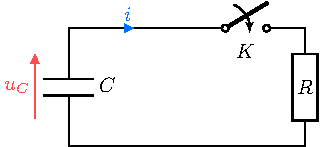
\includegraphics[width=\linewidth]{circuit_plain}
			\captionof{figure}{Circuit étudié.}
			\label{fig:circuit_plain}
		\end{center}
	\end{minipage}
}

\QR[6]{
	Déterminer qualitativement l'expression de la tension $v$ à basse fréquence
	puis à haute fréquence. On utilisera pour cela les schémas équivalents pour
	les fréquences concernées. Quel est le type de filtre correspondant à cette
	situation~?
}{
	En basse et haute fréquence, on a les schémas équivalents suivants~:
	\smallbreak
	\noindent
	\begin{minipage}[t]{.48\linewidth}
		~
		\begin{center}
			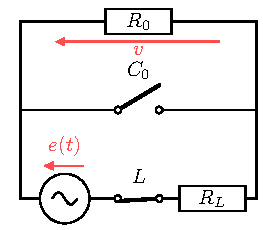
\includegraphics[width=.7\linewidth]{circuit_BF}
			\captionof{figure}{Basses fréquences\protect\pt{1}.}
			\label{fig:BF}
		\end{center}
		Ainsi, à basse fréquence, en appliquant un pont diviseur de tension
		\pt{1}, on a
		\[
			\xul{v} \stm{=} \dfrac{R_0}{R_0+R_L}\xul{e} \approx \eu
		\]
		puisque $R_0 \gg R_L$.
	\end{minipage}
	\hfill
	\begin{minipage}[t]{.48\linewidth}
		~
		\begin{center}
			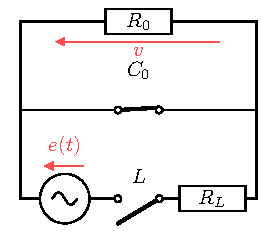
\includegraphics[width=.7\linewidth]{circuit_HF}
			\captionof{figure}{Hautes fréquences\protect\pt{1}.}
			\label{fig:HF}
		\end{center}
		À haute fréquence,
		\[
			\xul{v} \stm{=} 0
		\]
		car c'est la tension aux bornes d'un fil.
	\end{minipage}
	\smallbreak
	Le circuit se comporte donc comme un \textbf{filtre passe-bas} \pt{1}.
}

\QR[4]{
	Déterminer, en fonction des données, de l'inductance de la bobine $L$ et de la
	pulsation $\w$, la fonction de transfert complexe $\Hu(\w) = \frac{\Vu}{\Eu}$
	où $\Vu$ et $\Eu$ sont les amplitudes complexes associées aux signaux $v(t)$
	et $e(t)$. La mettre sous la forme $\Hu = \frac{1}{\ldots}$.
}{
	L'association parallèle du condensateur et de la résistance $R_0$ est
	équivalente à une admittance $\xul{Y}\ind{eq}\stm[-1]{=}\jj
		C_0\w+\frac{1}{R_0}$. On applique ensuite un pont diviseur de tension~:
	\begin{DispWithArrows*}
		\Vu &\stm{=} \frac{\Zu\ind{eq}}{\Zu\ind{eq}+\Zu_{R_L}+\Zu_{L}}\Eu
		\CArrow{$\times \frac{\Yu\ind{eq}}{\Yu\ind{eq}}$}
		\\\Lra
		\Hu = \frac{\Vu}{\Eu} &\stm{=} \frac{1}{1+(R_L+\jlw)\xul{Y}\ind{eq}}
		\Arrow{On remplace}
		\\\Lra
		\Hu &= \frac{1}{1+(R_L+\jlw)(\jj C_0\w+\frac{1}{R_0})}
		\Arrow{On développe}
		\\\Lra
		\Aboxed{
			\Hu &\stm{=} \frac{1}{1+\frac{R_L}{R_0} - LC_0\w^2 +
				\jw\left(R_LC_0+\frac{L}{R_0}\right)}
		}
	\end{DispWithArrows*}
}

\enonce{
	On rappelle les formes canoniques pour deux types de filtre d'ordre 2~:
	\begin{align*}
		\Hu=\frac{H_0}{1-x^2+\frac{\jx}{Q}}    & \quad \text{(passe-bas)}   \\
		\Hu=\frac{H_0}{1+\jj Q(x-\frac{1}{x})} & \quad \text{(passe-bande)}
	\end{align*}
	avec $x=\frac{\w}{\w_0}$ la pulsation réduite et $Q$ le facteur de qualité.
}

\QR{\label{q:w}
	Écrire la fonction de transfert précédente sous la forme canonique appropriée.
	En déduire le facteur de qualité et la pulsation propre $\w_0$ en fonction de
	$C_0$, $R_0$, $R_L$, et $L$.
}{
	On a $1+\frac{R_L}{R_0}=\frac{R_0+R_L}{R_0}$. On multiplie en haut et en bas
	\pt{1} l'expression de $\Hu$ par $\frac{R_0}{R_0+R_L}$~:
	\[
		\Hu \stm{=} \frac{\frac{R_0}{R_0+R_L}}
		{1 - \frac{LC_0R_0}{R_0+R_L}\w^2 +
			\jw\frac{R_0}{R_0+R_L}\pa{R_LC_0+\frac{L}{R_0}}}
	\]
	On a donc la forme canonique souhaitée (celle du passe-bas du second ordre)~:
	$\Hu=\dfrac{H_0}{1-x^2+\frac{\jx}{Q}}$ avec
	\[
		\boxed{H_0 \stm{=} \frac{R_0}{R_0+R_L}}
		\qet
		\w_0^2 = \frac{R_0+R_L}{LCR_0}
		\Ra
		\boxed{\w_0 \stm[-1]{=} \sqrt{\frac{R_0+R_L}{LC_0R_0} }}
	\]
	On en déduit le facteur de qualité par identification~:
	\begin{DispWithArrows*}[]
		\frac{1}{Q\w_0} &\stm{=} \frac{R_0}{R_0+R_L}\pa{R_LC_0+\frac{L}{R_0}}
		\Arrow{On développe}
		\\\Lra
		\frac{1}{Q\w_0} &= \frac{R_LR_0C_0 + L}{R_L+R_0}
		\CArrow{$(\cdot )^{-1}$}
		\\\Lra
		\w_0 Q &= \frac{R_L+R_0}{R_LC_0R_0+L}
		\CArrow{$\mdiv \w_0$}
		\\\Lra
		Q &\stm{=} \frac{R_L+R_0}{R_LC_0R_0+L}\frac{1}{\w_0}
		\Arrow{On remplace}
		\\\Lra
		Q &= \frac{R_L+R_0}{R_LC_0R_0+L}\sqrt{\frac{LC_0R_0}{R_0+R_L} }
		\Arrow{On simplifie la racine}
		\\\Lra
		\Aboxed{Q &\stm[-1]{=} \frac{\sqrt{(R_L+R_0)LC_0R_0}}{R_LC_0R_0+L}}
	\end{DispWithArrows*}
}

\enonce{
	Dans toute la suite, on utilisera la forme canonique.
}


\QR{
	\'Etablir la condition d'existence d'une résonance et déterminer la pulsation de résonance  $\w_r$ en fonction du facteur de qualité et de la pulsation propre.
}{
	Par définition,
	\eq{
		G=|\Hu|=\frac{|H_0|}{\sqrt{(1-x^2)^2+\frac{x^2}{Q^2}}}
	}

	Comme le numérateur est constant, cette fonction est maximale si le dénominateur est minimal. Par ailleurs, la fonction racine étant monotone croissante, on peut alors chercher le minimum de la fonction
	\eq{
		f:x \to (1-x^2)^2+\frac{x^2}{Q^2}
	}

	sur $\mathbb{R}^{+\star}$. Pour cela, on dérive et on cherche la valeur d'annulation~:
	\eq[align*]{
		f'(x)&=2(-2x)(1-x^2)+\frac{2x}{Q^2} \\
		\text{or}\, & f'(x)=0 \quad \Ra \quad 2(2x)(1-x^2)=\frac{2x}{Q^2}
	}

	On cherche une solution non nulle, on en déduit
	\eq{
		2(1-x^2)=\frac{1}{Q^2} \quad \Ra \quad  1-x^2=\frac{1}{2Q^2} \Ra x^2=1-\frac{1}{2Q^2}
	}

	Cette équation n'admet de solution que si $1-\frac{1}{2Q^2}\geq 0$, soit si $Q\geq \frac{1}{\sqrt{2}}$.

	Le gain présente donc un maximum autre que celui obtenu en basse fréquence si et seulement si $\boxed{Q\geq \frac{1}{\sqrt{2}}}$. Il s'agit de la condition de résonance. Le gain est alors maximal en $\boxed{x_r=\sqrt{1-\frac{1}{2Q^2}}<1}$
}


\QR{
	Tracer l'allure de $G=|\Hu|$ en fonction de la pulsation réduite $x$ dans le cas où il y a résonance.
}{

	\noindent
	\begin{minipage}[c]{.49\linewidth}
		En basses fréquences, $x\ll 1$ donc $\Hu=\frac{H_0}{1-x^2+\jj \frac{x}{Q}}\approx H_0$. On a donc $G=|H_0|=cte$
		\par
		En hautes fréquences, $x\gg 1$ donc $\Hu=\frac{H_0}{1-x^2+\jj\frac{x}{Q}}\approx \frac{H_0}{-x^2}$. On a donc $G=\frac{|H_0|}{x^2}\propto\frac{1}{x^2}$
		\par
		\medskip
		De plus, on a $G(\w_0) = H_0 Q > H_0$ en cas de résonance marquée. On en déduit l'allure ci-contre.
	\end{minipage}
	\hfill
	\begin{minipage}[c]{.49\linewidth}
		~
		\begin{center}
			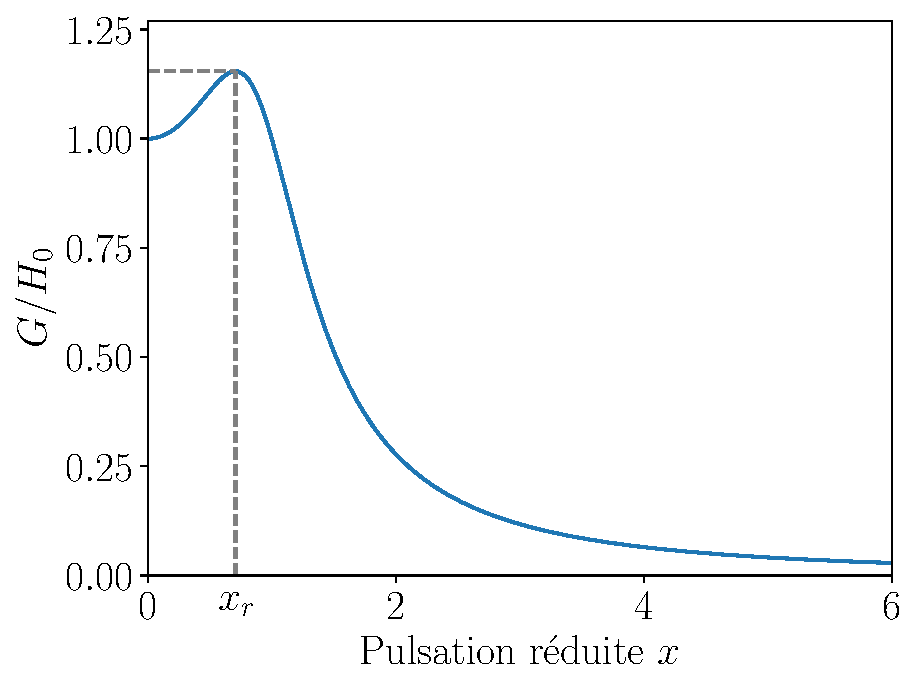
\includegraphics[width=\linewidth]{gain.pdf}
			\captionof{figure}{Gain en fonction de la pulsation réduite $x$}
			\label{fig:gain}
		\end{center}
	\end{minipage}
}

\enonce{
	Dans les questions suivantes, on suppose que le facteur de qualité est grand.
	La réponse expérimentale du microphone (amplitude de la tension $v$ en
	fonction de la fréquence $f$ pour une amplitude de tension d'entrée constante)
	est donnée par la courbe ci-dessous. On propose d'étudier trois méthodes pour
	estimer le facteur de qualité à l'aide de cette courbe.
	\begin{figure}[htbp!]
		\centering
		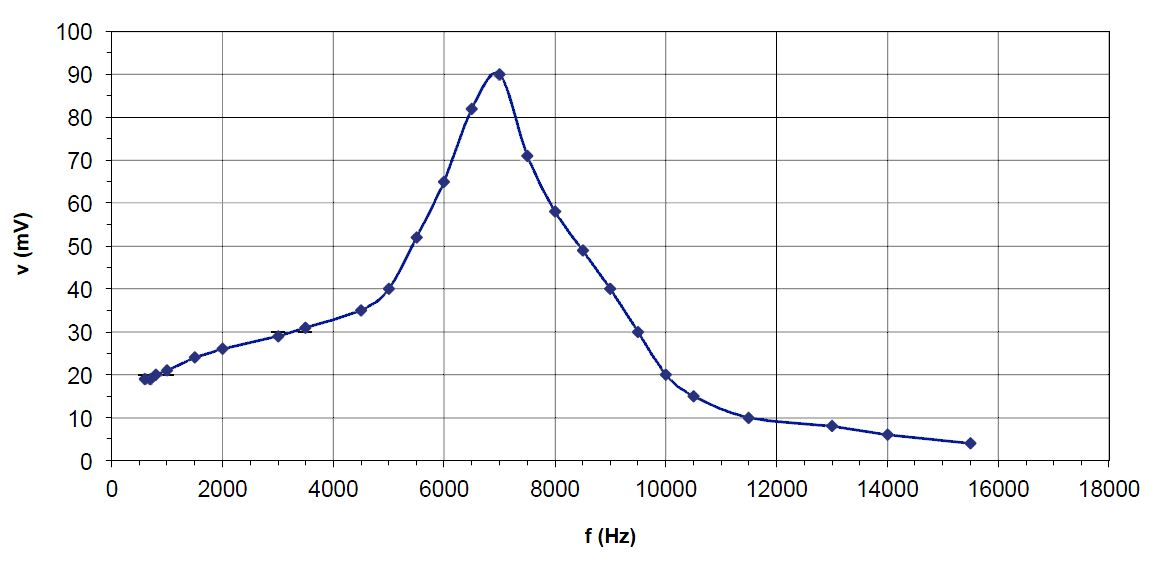
\includegraphics[width=\linewidth]{bode.jpg}
		\caption{Diagramme de \textsc{Bode} expérimental.}
		\label{fig:ddb}
	\end{figure}
}

\QR{
	Comment se simplifie l'expression de la pulsation de résonance lorsque $Q\gg 1$.  Exprimer la valeur maximale du gain $G_{\max}$ en fonction du facteur de qualité et de $H_0$.
}{
	Si $Q\gg 1$, $\frac{1}{Q^2}\ll 1$ donc $x_r=\sqrt{1-\frac{1}{2Q^2}}\approx 1$. Ainsi, $\boxed{\w_r=\w_0}$

	On a alors
	\eq{
		G_{max}=G(x=1)=\left|\frac{H_0}{1-1+\jj\frac{1}{Q}}\right| \Ra \boxed{G_{max}={H_0Q}}
	}

}

\QR{
%	Où peut-on lire $H_0$~? En déduire après lecture graphique une valeur numérique pour $Q$.
Par analyse du graphique, déterminer une valeur numérique pour $Q$.
}{
$H_0=G_{BF}$. On a donc
\eq{
	\boxed{Q=\frac{G_{\max}}{G_{BF}}}
}

Sur le graphique, on lit $G_{\max} / G_{BF} = v_{\max} / v_0 = 90/19$. Il vient donc $Q=\frac{90}{19} \approx 4,5$. Avec un seul chiffre significatif~: $\boxed{Q=5}$.
}

\enonce{
	On définit l'acuité $A$ de la résonance par la relation suivante~:
	\eq{
		A = \frac{f_r}{\Delta f} \approx Q
	}

	avec $\Delta f$ la largeur de la bande passante.
	On admet que $A$  est égal à $Q$ dans le cas étudié ici.
}


\QR{
	Rappeler la définition d'une fréquence de coupure.
}{
	Une fréquence de coupure $f_c$ est telle que $\boxed{G(f_c)=\dfrac{G_{max}}{\sqrt{2}}}$, ou avec la tension $\boxed{v(f_c)=\dfrac{v_{max}}{\sqrt{2}}}$
}


\QR{
	Faire une seconde estimation du facteur de résonance à l'aide d'une mesure de l'acuité.
}{
	Sur le graphique, on relève $f_r=\SI{7000}{Hz}$. On détermine les fréquences de coupure en cherchant les points où $v=\frac{v_{max}}{\sqrt{2}}=\frac{90}{\sqrt{2}}=\SI{64}{mV}$.

	On lit $f_{c1}=\SI{6,00}{kHz}$ et $f_{c2}=\SI{7,50}{kHz}$. On a donc
	\eq{
		A=Q=\frac{7000}{1,50.10^3}\approx 4,67
	}

	Avec un chiffre significatif~: $\boxed{Q=5}$. On retrouve bien le même résultat qu'avec l'autre méthode.
}


\QR{
	À l'aide des expressions de $\w_0$ et $Q$ déterminées dans la question \ref{q:w}, donner une estimation de la valeur de l'inductance $L$ à partir d'une lecture graphique de la fréquence de résonance $f_r$. En déduire le facteur de qualité puis commenter le résultat obtenu.
}{
	La lecture de $f_0$ nous donne $\w_0$. Or, $\w_0=\sqrt{\frac{R_0+R_L}{LC_0R_0} }$ d'où
	\eq[align*]{
		& \w_0^2=\frac{R_0+R_L}{LC_0R_0} \\
		\Ra & \boxed{L=\frac{R_0+R_L}{C_0R_0\w_0^2}=\frac{R_0+R_L}{4\pi^2 f_0^2 C_0R_0}}
	}

	Or, comme $R_L=\SI{3e3}{\ohm}$ et $R_0=\SI{1e6}{\ohm}$, on peut considérer que $R_L\ll R_0$, on a alors $R_L+R_0\approx R_0$ d'où
	\eq{
		\boxed{L=\frac{1}{4\pi^2 f_0^2 C_0}}
	}

	%	L'application numérique, en ordre de grandeur, donne
	%	\eq{
	%		L=\frac{1}{4.(7.10^{3})^2 10^{-10}}{0,3^2} H \approx \frac{1}{4 .49.10^{-4}}{9.10^{-2}} H =\frac{1}{200.10^{-4}}10^{-1} H=\frac{1}{2}10^{1}H\approx \SI{5}{H}
	%	}
	%	Soit \underline{$L=\SI{5}{H}$}.

	L'application numérique donne
	\eq{
		L=\frac{1}{4\pi^2 (7.10^{3})^2 10^{-10}}
		\qsoit
		\boxed{L=\SI{5}{H}}
	}


	On peut alors retrouver $Q$ en appliquant la formule théorique provenant de la détermination de la fonction de transfert~:
	\eq{
		Q = \frac{\sqrt{(R_L+R_0)LCR_0}}{R_LCR_0+L}\approx \frac{\sqrt{LCR_0^2}}{R_LCR_0+L} \approx 4
	}

	D'où finalement $\boxed{Q \approx 4}$
	On obtient bien des résultats cohérents avec les 3 méthodes. Le facteur de qualité est relativement grand devant 1, ce qui est cohérent avec l'hypothèse faite au début de l'étude.
}


\QR{
	La fréquence de résonance varie selon le type de microphone utilisé. Quel est l'effet sur le son restitué~?
}{
	Le microphone est un passe-bas mais du fait de son facteur de qualité élevé, il possède une résonance marquée. Pour une même note jouée par l'instrument, l'usage de deux microphones différents induira la restitution de la même \textbf{note} (caractérisée par la fréquence du fondamental et sachant qu'un filtre linéaire ne modifie jamais la fréquence fondamentale du signal), mais le spectre sera différent car toutes les harmoniques ne seront pas amplifiées de la même façon suivant la valeur de la fréquence de résonance. Le type de microphone modifie donc le \textbf{timbre} du son. Le choix du microphone peut donc donner un son plus "jazz" ou plus "rock"...
}


\end{document}
